\note{Brief Overview} {
	The first \CLASP{} Activity, \ref{act1.1.6}, based on \ref{FNT1.1.3-4}, \ref{FNT1.1.3-5}, \ref{FNT1.1.3-6} provides a good review of the qualitative application of both the \ThreePhaseModel{} and the \EnergyInteractionModel{}. You should now be feeling fairly confident with this material. The second Activity, \ref{act1.1.7} based on \ref{FNT1.1.4-1} and \ref{FNT1.1.4-2} apply the \EnergyInteractionModel{} to chemical reactions. 

The last \CLASP{} Activity continues Module 1.2: Getting Quantitative with Models is a follow-up of \ref{FNT1.2.1-1}, \ref{FNT1.2.1-2}, \ref{FNT1.2.1-3}, \ref{FNT1.2.1-4}.
	
\section*{\CLASP{} Activities}
	
\subsection*{\ref{act1.1.6} Making Sure Things are Making Sense	(\about\unit[35]{min})}
	
\subsubsection*{Purpose}

\begin{itemize}
	\item To provide more additional practice applying both the \ThreePhaseModel{} and the \EnergyInteractionModel{} to fairly simple thermal phenomena.
	\item To provide an opportunity for students to make sure they have gotten the basics of applying these two models.
\end{itemize}

\subsubsection*{Learning Outcomes}
\begin{itemize}
	\item Confidence in being able to apply the two models to simple thermal phenomena.
\end{itemize}

}
%%%%%%


\section{Refining Intuitions through Practice}
\label{act1.1.6}

\begin{overview}

	\noindent
	{\bfseries Overview:} Remember how we \hyperref[ReadingRefiningIntuitions]{talked about ``refining intuitions''} and becoming so familiar with using our models that they become ``second nature'' to us? For that to happen, we need to practice using our models even more. This is what the following activities are all about. We'll attempt to make sense of more thermal phenomena by using the \ThreePhaseModel{} and the \EnergyInteractionModel{}, so that we'll become able to intuitively use them in new situations.
	
\end{overview}
\note{Brief Overview}{
The first \CLASP{} Activity, \ref{act1.1.6}, based on \ref{FNT1.1.3-4}, \ref{FNT1.1.3-5}, \ref{FNT1.1.3-6} provides a good review of the qualitative application of both the \ThreePhaseModel{} and the \EnergyInteractionModel{}. You should now be feeling fairly confident with this material. The second Activity, \ref{act1.1.7} based on \ref{FNT1.1.4-1} and \ref{FNT1.1.4-2} apply the \EnergyInteractionModel{} to chemical reactions. The last \CLASP{} Activity continues Module 1.2: Getting Quantitative with Models is a follow-up of \ref{FNT1.2.1-1}, \ref{FNT1.2.1-2}, \ref{FNT1.2.1-3}, \ref{FNT1.2.1-4}.
}



\subsection{Energy in ice and liquid water}

\note{Timing: \unit[\textless5]{min}}{
	\subsubsection*{Principal learning goal}
	To learn to use the model to develop an answer that may not be immediately obvious by translating the process or situation in question into the ``language'' of the model, often in the form of a diagram, and then searching for implications or inconsistencies based on the logic of the model.
}

\begin{FNTenv}
	\input{U1/FNT1.1.3-4}
\end{FNTenv}

\noindent Make an \EnergyDiagram{} that relates the initial and final states described in the \FNT{}. Use the diagram, and the logic of the model to explain which state would have more total energy.

\note{Answer to question}{
	By using an \EnergyDiagram{}, it should be obvious that energy had to be added to the ice to break some bonds (bond energy went up), while the thermal energy is unchanged (according to the simple version of our model, which we extend when we develop a particle model of bond and thermal energy), so the liquid water has more energy.
}
\note{FYI}{
	There is often a change of thermal energy at a phase change, due to a change in the heat capacity, but we are ignoring this for now in our simple model.  Don't bring this up with the students yet.  Everyone will eventually be able to deal with several subtle aspects like this, but not until we have mastered some basic thermodynamic relationships.
}

\WCD
\note{}{
	Have one or two groups give a careful explanation using the logic of the model.  Every statement must come from the model or be justified in some way (logic of the model).  Students are not used to doing this.  Emphasize it.  This is often where students falter on quizzes.
}

\subsection{The physical concept of \emph{Heat}}

\note{Timing: \unit[\about1]{min}}{
	\subsubsection*{Purpose}
	
	To emphasize the importance of knowing and using correct definitions of technical terms. In this case, the technical term is ``heat'' and how it is now used in both chemistry and physics texts, in contrast to how it was used historically.
}

\begin{FNTenv}
	\input{U1/FNT1.1.3-5}
\end{FNTenv}

\noindent Discuss your response for this \FNT{} with your group mates. Make sure everyone in your group is prepared to explain to the whole class. This is a group responsibility!

\note{Optimal response}{
	The important point is that ``heat'' has a technical definition that is much more restricted than its use in everyday English. Heat is a {\em transfer} of energy between two physical things as a result of a temperature difference between them.
}

\WCD
\note{}{
	Give them a couple of minutes to discuss in their Small Groups (SG), and have someone explain to the Whole Class.  You should comment that historically, the word ``heat'' was often used for what we now call thermal energy.  Some older textbooks will use ``heat'' this way.  This is one of those cases where you need to read critically, to know how a word is being used.  All newer introductory textbooks in both chemistry and physics we are aware of, however, use the term ``heat'' as we have defined it here.
}

\subsection{Equilibrating Copper and Water}

\note{Timing: \unit[\about20]{min} total for all parts, not including \WC{} discussions}{
	Notice that there are two \WC{} discussions, one after they put parts 1 and 2 on the board, and then one after they respond to part 3.
}

\begin{FNTenv}
	\input{U1/FNT1.1.3-6}
\end{FNTenv}

\begin{enumerate}
	\item Put your \TempGraphs{} on the board with the initial state marked on each one. Explain briefly how you can tell if either substance might undergo a phase change during this process.
	
	\note{For example}{
		``Given the initial states on a \TempGraph{}, neither substance will reach a phase change temperature as energy in the form of heat is transferred between them'', or, ``There are no phase change temperatures for either substance in the range of possible final temperatures.''
	}

	\item Put your complete \EnergyDiagram{} on the board for this process.
	
	If ${\Delta E_\text{thermal(Cu)} = \text{\unit[250]{kJ}}}$, what is $\Delta E_{\text{thermal}\left(\text{H}_2\text{O}\right)}$? Explain why.
	
	\note{}{
		\noindent
		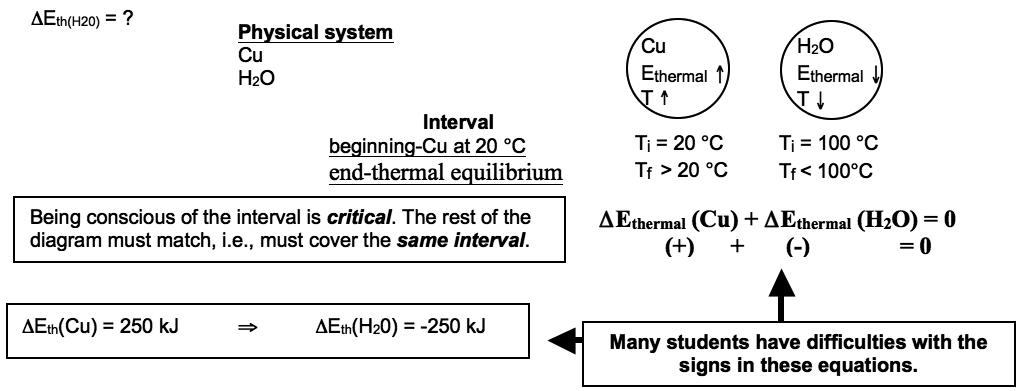
\includegraphics[width=\linewidth]{act116-b}
	}
	
\WCD

	\note{}{
		Do any clarifying that is necessary, but try to get the students to do most of the explaining. 
		
		At the end of this whole-class discussion, ask the question: ``Why was it necessary to ask part (b) after part (a) and not vice-versa?''
		
		Answer: To apply the \EnergyInteractionModel{} you have to know what energy systems are involved.  In this particular case, that means knowing whether or not there will be a phase change of either of the substances.  
	}
	
	\item Redraw your \TempGraphs{} for the new initial conditions. Explain briefly how you could determine if the \ce{H2O} will undergo a phase change or temperature change.
	
	\note{The students will need to be able to do this kind of analysis in \DLM03!}{
		\todo[inline]{What is this reference to \DLM03 in \DLM4 using future tense about?}
		Help them figure out that they need to compare the magnitude of energy needed to increase the temperature of the Cu to 100$^\circ$C with the magnitude of energy lost by the \ce{H2O} as it completes its phase change to decide if the \ce{H2O} will change temperature.
		\begin{itemize}
			\item If the former is smaller, when the Cu reaches 100$^\circ$C the \ce{H2O} will only be partway through its phase change, and the process will stop (thermal equilibrium). 
			\item If the former is larger, the \ce{H2O} will complete its phase change before the Cu reaches 100$^\circ$, and the process will continue until thermal equilibrium is reached. 
		\end{itemize}
	}
\end{enumerate}

\WCD

\note{}{
	Try to get the students to do most of the explaining, but make sure all of the important points are covered.
}